\chapter{Design}\label{C:design}

\vspace{-3mm}

\begin{figure}[H]
    \begin{center}
        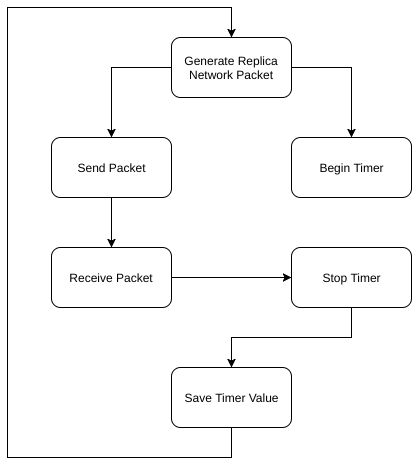
\includegraphics[keepaspectratio,width=8cm]{Images/MeasurementSequence}
        \caption{High level flow chart of Measurement Sequence}
        \label{fig:measurementsequence}
    \end{center}
\end{figure}


The goal of this project is to create a device which can measure latency between two connections with high precision
and accuracy. Figure \ref{fig:measurementsequence} shows the high level overview of what the device needs to be able 
to do. The following is the design decisions made to achieve the goal.

\section{Hardware Design}

For a platform to be flexible, it must be able to interact with any type of software and analysis tools. This is 
easily done by storing the data in an easy to use format (such as CSV) and providing it on a medium which is 
easily accessible and compatible with existing computers, which are typically x86 based PCs. Therefore, the choice 
was made to write the data to an SD card, which can be removed and inserted into a computer for post processing, 
allowing the platform to be flexible. 

At the same time as being a flexible platform, the device needs to be able to measure low level electrical signals 
with high reliability, while performing complex high-level instructions such as measuring the time between two 
signals. The best way to perform high precision actions with complex digital logic is a FPGA. The high-speed clocks 
involved with very precise timing instruments are too fast for a typical microcontroller or processor. 

A platform that combines both flexibility and ability to measure low level electrical signals is the Zynq line of 
FPGAs by Xilinx. These combine both a FPGA with an ARM processor, to allow for a full operating system to be run in 
tandem with operations on the FPGA.  The ARM processor can allow for future extensions onto the device to allow for 
interconnectivity with different kinds of storage mediums, and even connect to the internet too, making it a highly 
flexible platform. 

A FPGA System block must generate a network packet that can be used to measure the latency. On a x86 based computer, 
this is done through the CPU, and an element called a MAC. The MAC is used to convert logic link control signals 
into physical hardware signals for the Ethernet Phy to interpret. An Ethernet Phy is required as the 802.3ab 
standard defines the electrical connection from one node to another to consist of 4 twisted pairs and the 
differential electrical signals required for this cable is not possible in a FPGA, or in a CPU, hence this is 
offloaded to an external IC. Connections consist of commonly found Category 5e and 6 cabling, which adheres to the 
tolerance for how many twists are performed per meter cable (Important for signal integrity). The connection between 
the MAC and the Ethernet PHY is performed through a hardware protocol standard called Media Independent Interface 
(MII) and then converted to the differential signals across the Category 5e/6 cable. The gigabit version of ethernet 
uses an extended version of MII called Reduced Gigabit Media Independent Interface (RGMII).

\section{Block Design (Concept)}

\vspace{-3mm}

\begin{figure}[H]
    \begin{center}
        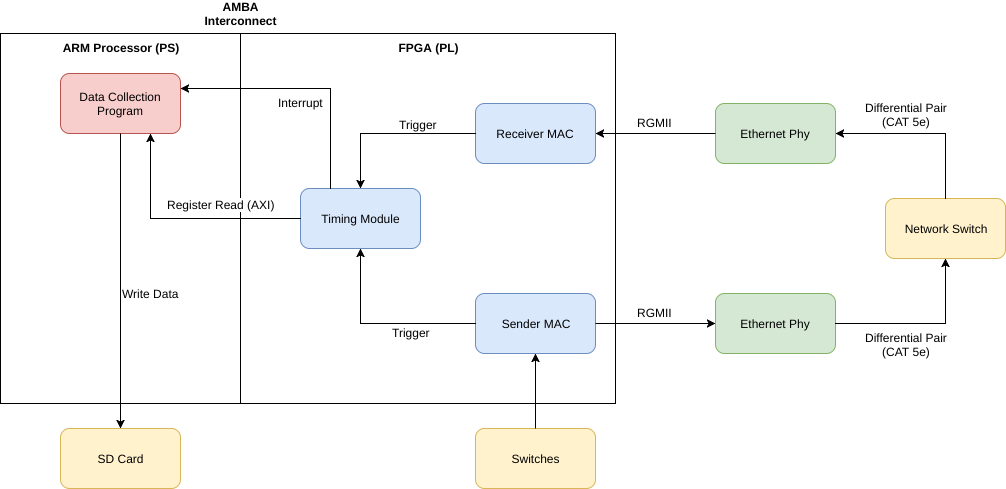
\includegraphics[keepaspectratio,width=15cm]{Images/BlockDesignConcept}
        \caption{Generic Block Design Concept. Blue represent FPGA logic blocks, Red represents Bare-Metal programs run on the ARM Processor, Green represents external ICs and Yellow represent other hardware external to the FPGA development board.}
        \label{fig:blockdesignconcept}
    \end{center}
\end{figure}

\vspace{-3mm}

\par The Sender MAC, the FPGA produces a repeated signal of a network packets and an interrupt to a timing module to 
begin counting. The number of packets per second (PPS) is controlled by hardware switches found on the development 
board itself. The Ethernet Phy converts these RGMII signals into differential signals what are used in communicating 
over CAT 5e/6 cable. This is then switched to the other Ethernet Phy, and the receiving end detects the incoming 
packet. The Receiver MAC detects the network packet, and produces an interrupt for the timing module to stop counting.

\par The Timing Module captures the events produced by the MACs and once a value is stored in the register, it 
produces an interrupt for the ARM Processor to begin reading the register. 

\par A program running on the ARM Processor intercepts the interrupt, and an interrupt service routine begins. This 
retrieves the value in the register and saves it to the SD card. Every time the interrupt is triggered, the value is 
appended to the end of a file stored on the SD Card. 

\section{Block Design (Implementation)}

\begin{figure}[H]
    \begin{center}
        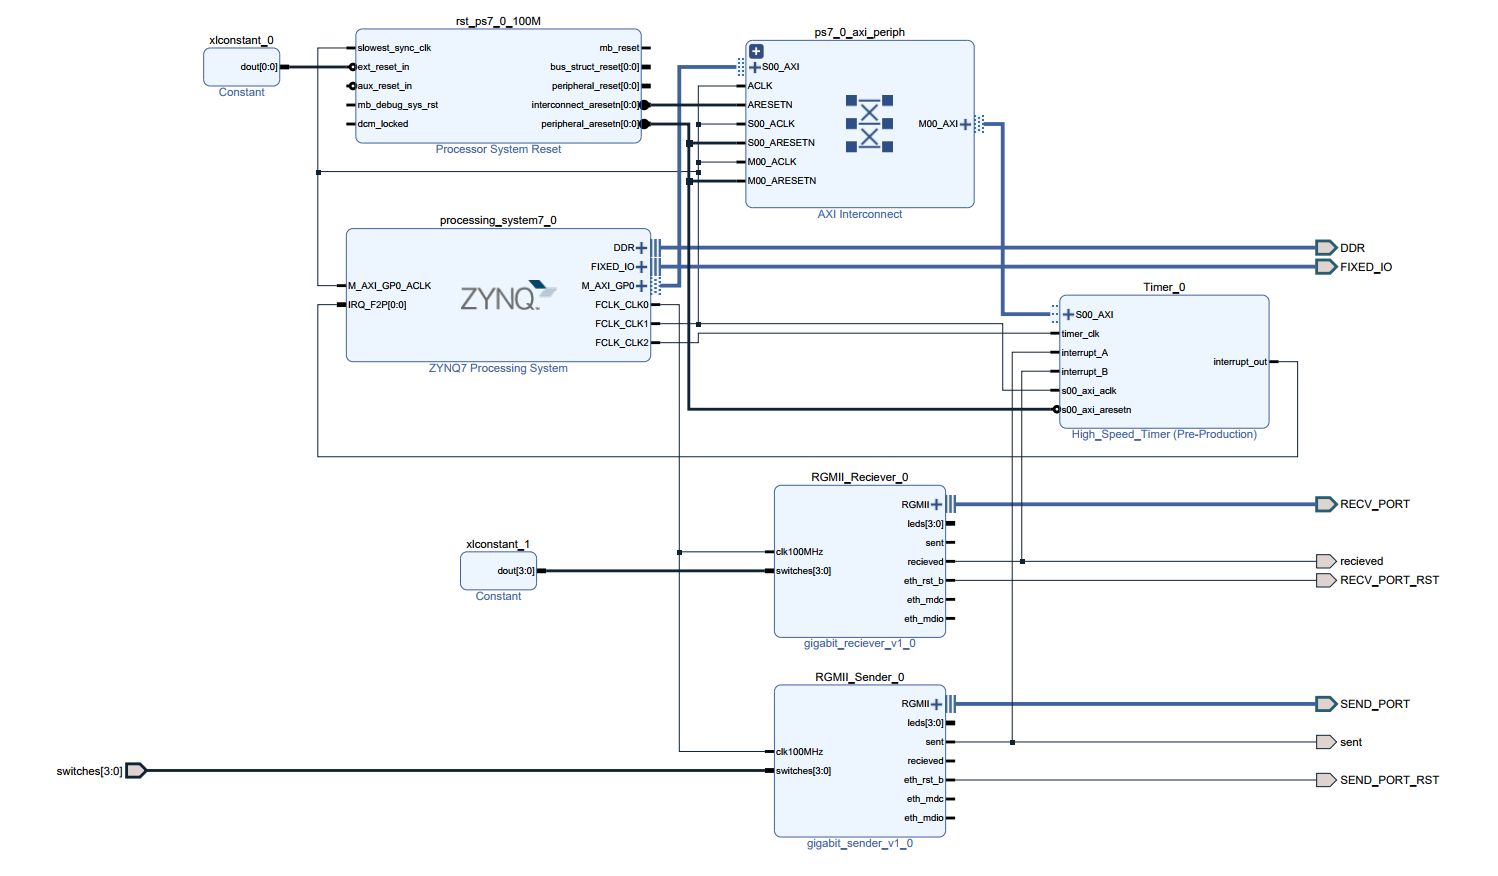
\includegraphics[keepaspectratio,width=15cm]{Images/BlockDesignImpl}
        \caption{FPGA Block Design Implementation. Each block is a VHDL module with the Input and Output exposed as 
        ports on the block itself.}
        \label{fig:blockdesignimpl}
    \end{center}
\end{figure}

\par Figure \ref{fig:blockdesignimpl} above shows the overall diagram of the FPGA logic blocks. This is the view 
through the IP integrator in Vivado 2017.2. Thicker lines in the diagram represent busses, while the thinner black 
lines represent single wires.  Connections on the left and right of the diagram represent Inputs and Outputs to the 
FPGA respectively. 

\par The extra blocks in the upper area of the diagram represent constructs needed for AXI peripherals. This allows 
the Processing Systen (PS) to interact and access registers found in the Programmable Logic (PL) of the FPGA. AXI manages the control signalling for buffering 
and clocking data in and out of the PS.

\section{Reduced Gigabit Media Independent Interface (RGMII)}

\par GMII is a full duplex interface between the MAC and an Ethernet Phy. As shown in Figure \ref{fig:gmiiwiring}, the physical wiring 
consists of 22 wires between the two devices. The signalling shown in Figure \ref{fig:gmiisignals} gives an example of how data is 
transferred to and from the Phy. Bytes transmitted to the Ethernet Phy are then converted and sent across the 
Cat5e/6 cable. RGMII is a Dual Data Rate Extension to GMII, by which the data is clocked on both the rising and 
falling edge of the clock. This means that one byte can be transmitted over four wires instead of 8, while keeping 
the same clock frequency. This is advantageous as there is commonly limited space on a PCB for wiring interconnects 
together, especially when there are more than 400 pins on a device (The XC7Z020-CLG484 has 
484 package pins). 

